\documentclass{ximera}

\newcommand{\RR}{\mathbb R}
\renewcommand{\d}{\,d}
\newcommand{\dd}[2][]{\frac{d #1}{d #2}}
\renewcommand{\l}{\ell}
\newcommand{\ddx}{\frac{d}{dx}}
\newcommand{\dfn}{\textbf}
\newcommand{\eval}[1]{\bigg[ #1 \bigg]}


\author{Jim Talamo}
\license{Creative Commons 3.0 By-bC}

\outcome{}

\begin{document}
\begin{exercise}
Suppose that $f(x) = \sum_{k=0}^{\infty} \frac{2^k}{2k-3}(x-2)^{3k+1}$.

\begin{exercise}
Find $f^{(16)}(2)$.

\[
f^{(16)}(2) = \answer{\frac{32}{7}} \cdot \left(\answer{16}\right)! 
\]
\end{exercise}

\begin{hint}
A good way to proceed is to use the relationship between the coefficients of the power series and the derivatives of the function it represents.

\[
\textrm{If } f(x) = \sum_{k=0}^{\infty} a_k(x-c)^k, \textrm{ then: } a_n = \frac{f^{(n)}(c)}{n!}
\]

Here, $c=\answer{2}$.  In order to find $f^{(16)}(2)$, we should use $n=\answer{16}$.

The coefficient in question is thus $a_{\answer{16}}$.  

\begin{question}
By definition $a_{16}$ is:

\begin{multipleChoice}
\choice{Always the coefficient obtained by plugging in $k=16$.}
\choice[correct]{The coefficient in front of $(x-c)^{16}$.}
\end{multipleChoice}

In this case, we find $(x-2)^{3k+1}=(x-2)^{16}$ when $k=\answer{5}$, so:

\[
a_{16} =  \frac{2^k}{2k-3} \bigg|_{k=\answer{5}} = \frac{\answer{32}}{\answer{7}}
\]

\begin{question}
We now use the formula $a_n = \frac{f^{(n)}(c)}{n!}$, with $n=16$ (as found earlier) to find:

\begin{align*}
a_{16} &= \frac{f^{(16)}(2)}{16!} \\
\answer{\frac{32}{7}} &= \frac{f^{(16)}(2)}{\left(\answer{16}\right)!}
\end{align*}

\begin{question}
Thus, $f^{(16)}(2) = \answer{\frac{32}{7}} \cdot \left(\answer{16}\right)! $

\end{question}
\end{question}
\end{question}

\end{hint}
%%%%%%%%%%%%%%
 
\begin{exercise}
Find $f^{(17)}(2)$.

\[
f^{(17)}(2) = \answer{0}
\]


\begin{hint}
A good way to proceed is to use the relationship between the coefficients of the power series and the derivatives of the function it represents.

\[
\textrm{If } f(x) = \sum_{k=0}^{\infty} a_k(x-c)^k, \textrm{ then: } a_n = \frac{f^{(n)}(c)}{n!}
\]

Here, $c=\answer{2}$.  In order to find $f^{(17)}(2)$, we should use $n=\answer{17}$.

The coefficient in question is thus $a_{\answer{17}}$.  

\begin{question}
By definition $a_{17}$ is:

\begin{multipleChoice}
\choice{Always the coefficient obtained by plugging in $k=17$.}
\choice[correct]{The coefficient in front of $(x-c)^{17}$.}
\end{multipleChoice}

In this case, we find $(x-2)^{3k+1}=(x-2)^{17}$ when $k=\answer{\frac{16}{3}}$.  

\begin{question}
Note that the index of summation only runs over integer values (i.e. $k=0,1,2,\ldots$). Since $k=\frac{16}{3}$ is not an integer:

\begin{multipleChoice}
\choice{$a_{17}$ is undefined.}
\choice[correct]{$a_{17}=0$.}
\end{multipleChoice}

\begin{question}
We now use the formula $a_n = \frac{f^{(n)}(c)}{n!}$, with $n=17$ (as found earlier) to find:

\begin{align*}
a_{17} &= \frac{f^{(17)}(2)}{17!} \\
\answer{0} &= \frac{f^{(17)}(2)}{\left(\answer{17}\right)!}
\end{align*}

Thus, $f^{(17)}(2) = \answer{0}$.
\end{question}
\end{question}
\end{question}
\end{hint}

\begin{exercise}
Of course, in this case, we could also write out the first several terms until we find the desired coefficients:

\begin{align*}
f(x) &=\sum_{k=0}^{\infty} \frac{2^k}{2k-3}(x-2)^{3k+1} \\
& = -\frac{1}{3} (x-2) +\answer{-2}(x-2)^4+\answer{4}(x-2)^7+\answer{\frac{8}{3}}(x-2)^{10}+ \\
& \qquad + \answer{\frac{16}{5}}(x-2)^{13}+\answer{\frac{32}{7}}(x-2)^{16}+\answer{\frac{64}{9}}(x-2)^{19}+\ldots \\
\end{align*}

Note that we obtain the coefficient $a_{16}$ when we substitute $k=5$ into the sum (as found earlier) and that the ``missing'' $(x-2)^{17}$ term should be thought of as $0 \cdot (x-2)^{17}$.  This is further justified via the observation:

\begin{image}
  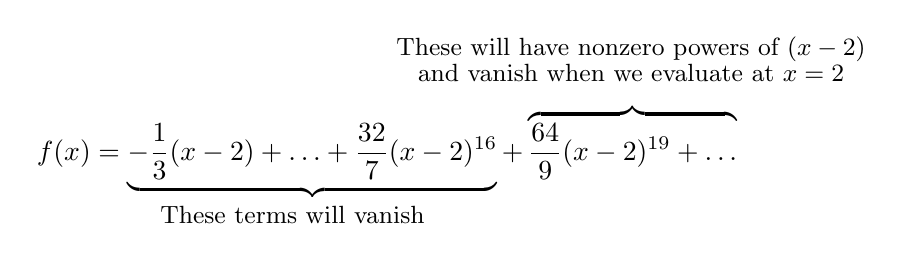
\begin{tikzpicture}
        \node at (0,0) {
          $f(x)= \underbrace{-\frac{1}{3}(x-2)+\ldots+\frac{32}{7}(x-2)^{16}}+ \overbrace{\frac{64}{9}(x-2)^{19}+\ldots}$};
        \node at (-1.2,-.8) {\small{These terms will vanish}}; 
        \node at (3.1,1.3) {\small{These will have nonzero powers of $(x-2)$}};  
        \node at (3.1,1) {\small{and vanish when we evaluate at $x=2$}};  
             \end{tikzpicture}
  \end{image}

Thus, there will be nothing nonzero left after taking $16$ derivatives and evaluating the result at $x=2$, so $f^{(17)}(2)$ should be $0$.


\end{exercise}
\end{exercise}

%%%%%%%%%%%%%%%%%%%






\end{exercise}
\end{document}
